\section{Design decisions}

\subsection{Database} \label{db_disc}
We used MongoDB to provide the database service. We chose to use this database as it is easy to implement and easy to use. We have a MongoDB database with 1 collection, \textit{Bikes}. The \textit{Bikes} collection stores all bike locations and their availability. There should be a second database collection, \textit{Users}, for storing the name, passwords and a list of rented bikes. In fact, we have implemented most of the back-end and front-end functionality to provide this, but due to the lack of time we weren't able to connect the front-end implementation with the back-end one.

The database entry for a bike looks as represented in \autoref{database}. Every bike has an automatically generated id, a pair of coordinates and a boolean availability status. The ids are unique for all the instances.

    \begin{figure}[H]
		\centering
		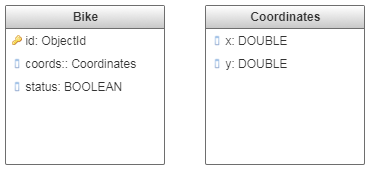
\includegraphics[width=0.7\textwidth]{images/db-structure.png}
		\caption{Bike model}
		\label{database}
	\end{figure}


In docker swarm mode, the Mongo replica set is used to enable sharing of the data between the instances of MongoDB on different hosts. Replica sets provide redundancy and increase the availability of the data. All write operations are performed to the primary node and then the data is replicated to the secondary nodes, as shown in \autoref{repl}. When communicating with the database, the driver is responsible for detecting the primary node. ReactiveMongo does not need any additional configuration for that and works perfectly both when there is a single instance of the database and a replica set.

    \begin{figure}[H]
		\centering
		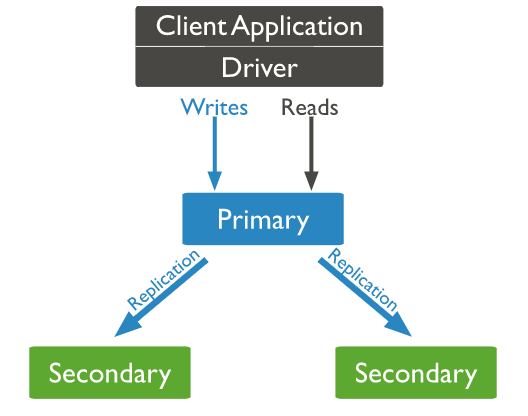
\includegraphics[width=0.7\textwidth]{images/replication.png}
		\caption{Replica sets in MongoDB}
		\label{repl}
	\end{figure}


As opposed to the other services that are deployed in docker swarm mode, MongoDB needs some additional configuration. Docker cannot take care of initializing the replica set and making sure that the data is correctly replicated among different nodes. This means that we have to manage the replica set ourselves. If the replica set is configured manually there is a high risk that if one of the MongoDB instances goes down and is then recreated again, its IP address will be different and the replica set will need to be reconfigured (the new IP address of the node should be added and the old one removed). This may cause read and write operations to fail, which is not what we want. So we have found a way to deal with this problem. We have a separate container (called \textit{controller}) that maintains the replica set up and running and updates the configuration whenever necessary.  This container does not need replication and is deployed only once on the manager node. So the backend, when deployed in swarm mode, looks as represented in \autoref{backend}.

    \begin{figure}[H]
		\centering
		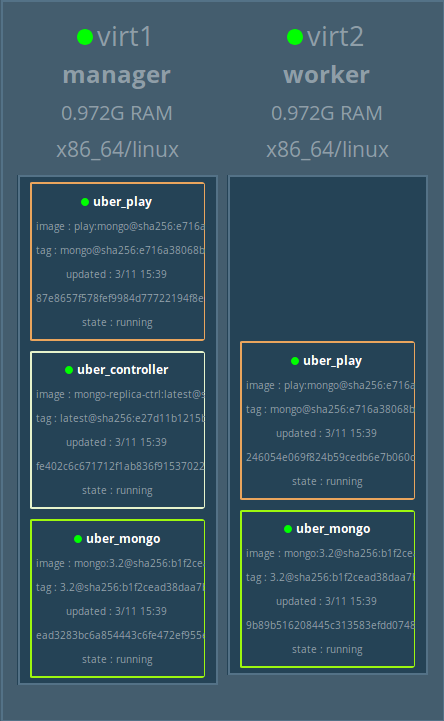
\includegraphics[width=0.7\textwidth]{images/backend.png}
		\caption{MongoDB replication in docker swarm mode}
		\label{backend}
	\end{figure}


\subsection{Webserver}
We chose Play as the framework for the back-end development of our application mostly because it supports asynchronous I/O. There were two main causes for choosing Scala: the first is the opportunity to learn a new programming language and the second is professor's incentive to use Scala for back-end development. In the end we succeeded in building a working back-end. We tried to benefit as much as possible from the completed projects we found on the Internet. They contributed a lot to our understanding of how everything needs to be done and to the development of the final product. During the development we had difficulties connecting different services (back-end, front-end, database) to each other as well as using WebSockets for live data streaming.

\subsection{Client}
Angular is a framework for building Web single-page applications and Bootstrap is an easy to use front-end web framework for designing web applications. These are the main reasons why we chose to use these frameworks. Other advantage of using Angular is its highly readable and comprehensive code. It was an important factor because we wanted something that would take as little time to learn as possible. We created the project using Angular Cli and used the corresponding components to create navigation bar, map component, and two (login and registration) forms (unfortunately not seen in the final layout). Even if it is not linked to the framework itself, we found the large community of developers using Angular extremely useful as online answers helped us solve most encountered problems.

\begin{figure}[H]
		\centering
		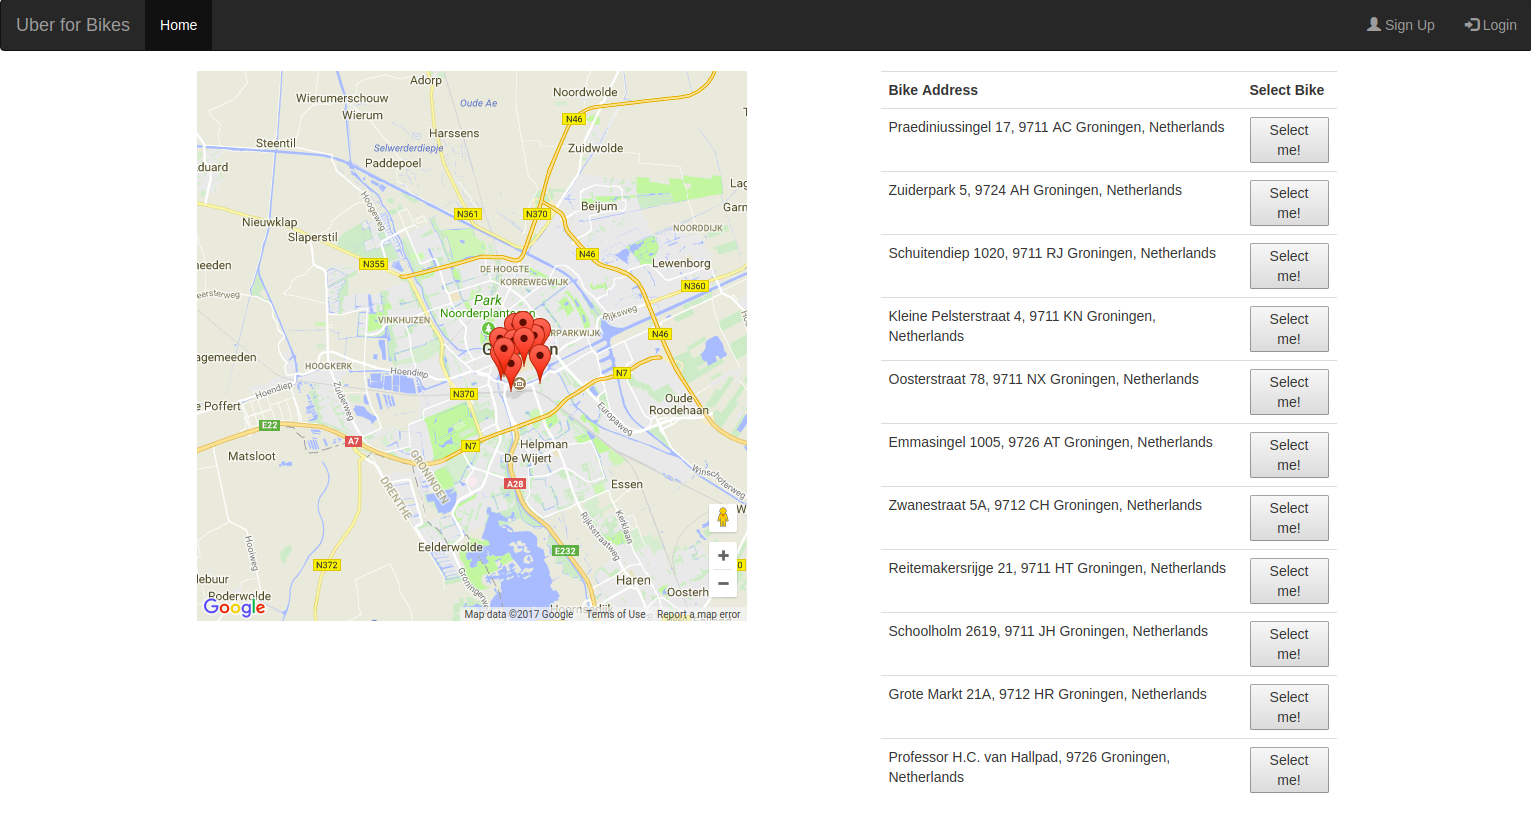
\includegraphics[width=\textwidth]{images/screenshot.png}
		\caption{Application layout}
		\label{front-end}
	\end{figure}
